\label{sec:experiments}


\begin{figure*}[t]
  \centering
  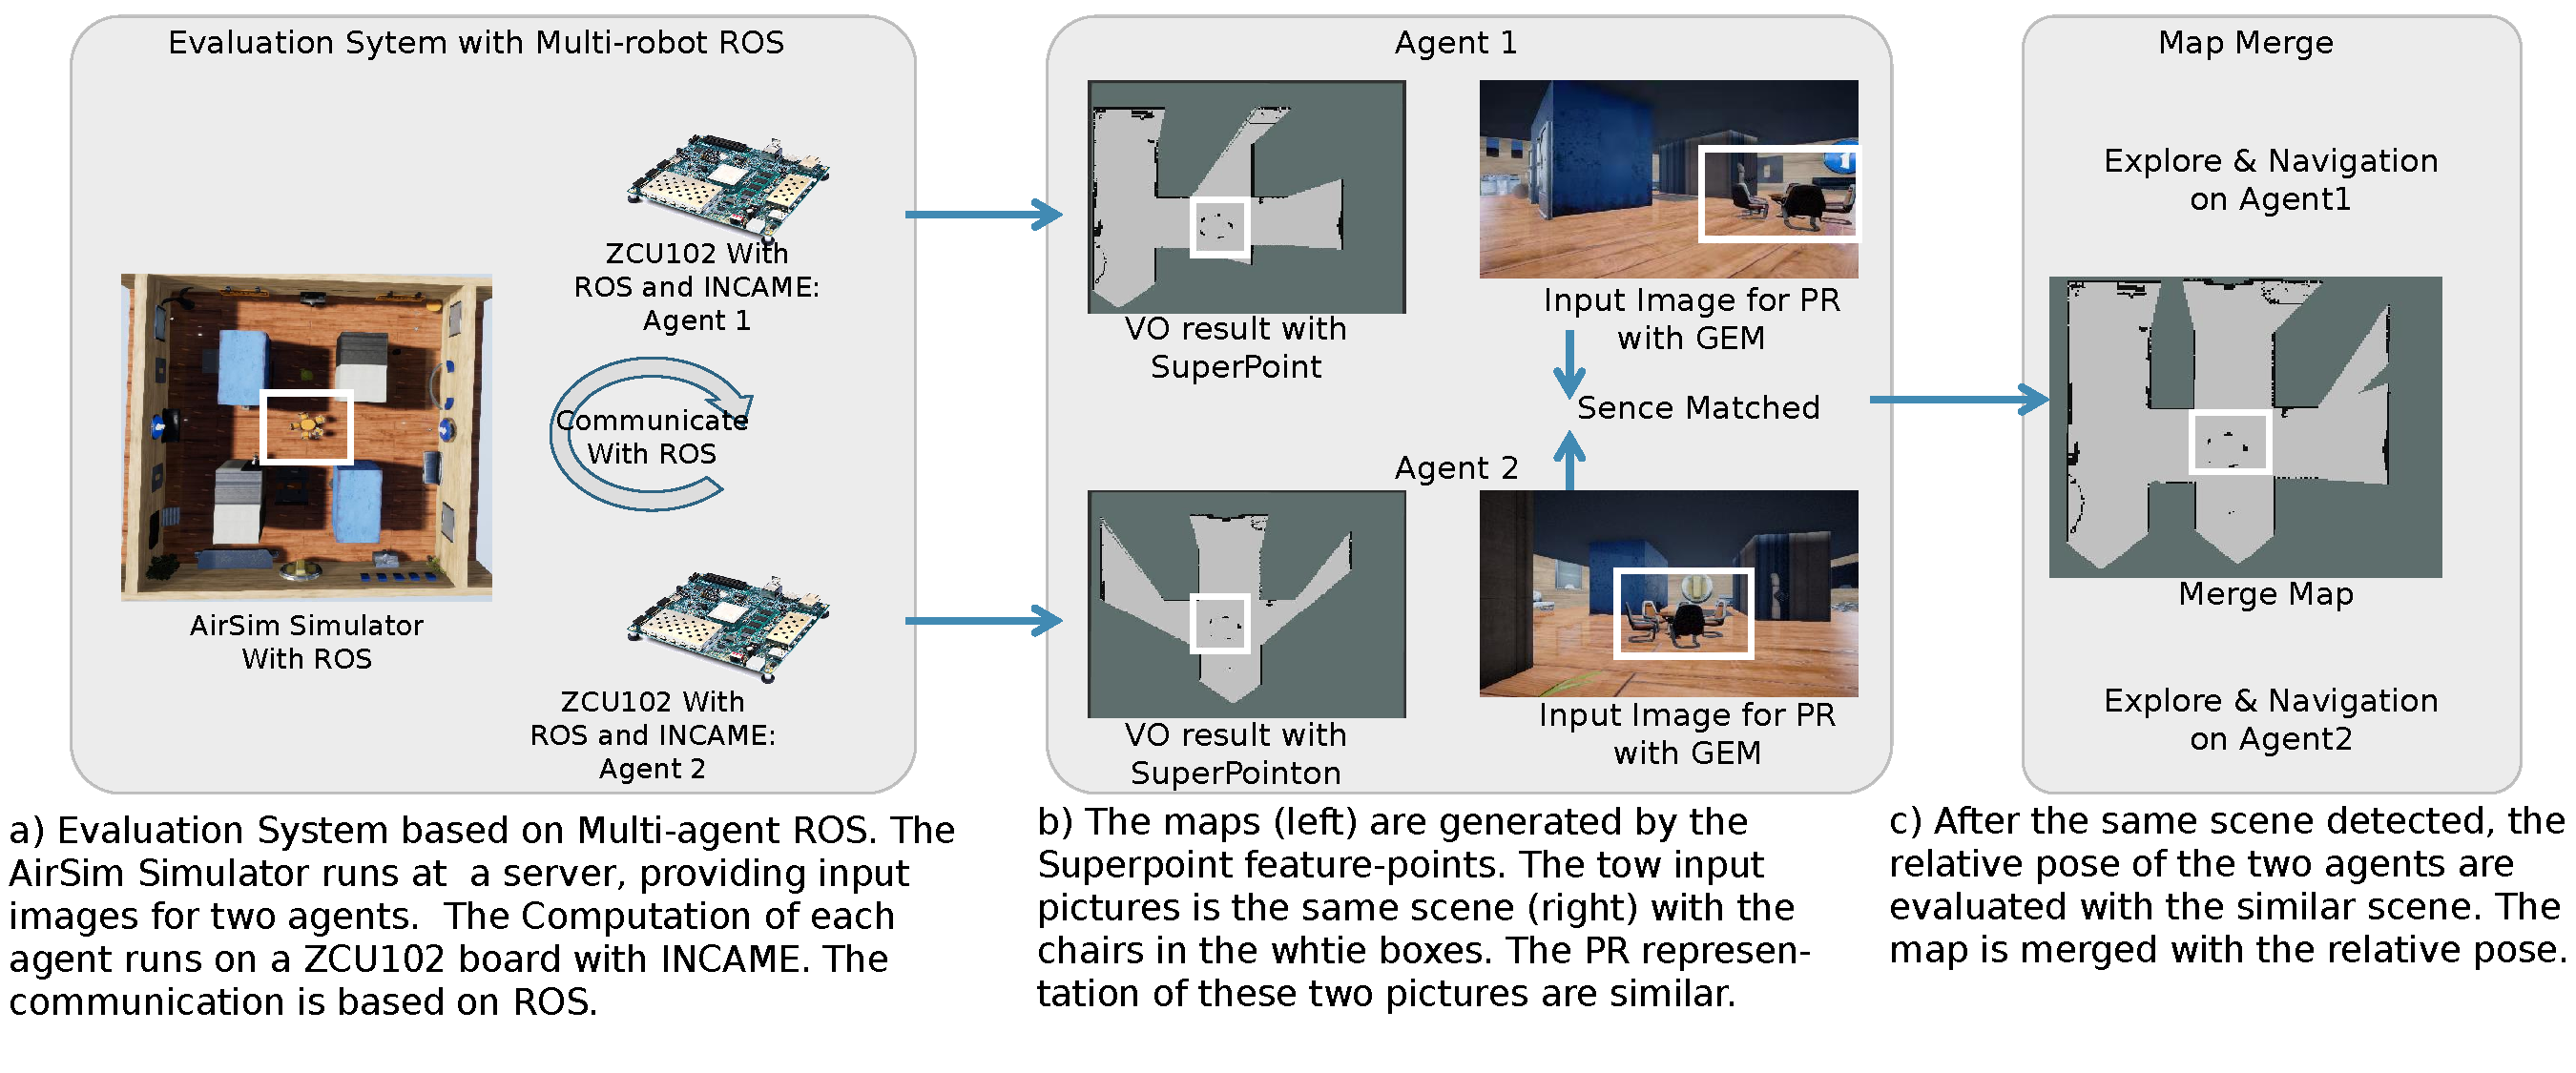
\includegraphics[width=0.9\linewidth]{fig/env.pdf}
  \caption{Muti-Robot Exploration: environment and results. }
  \label{fig:env}
\end{figure*}

In this section, the evaluation of the instruction-based-interruption, hardware modules for post-processing, and the overall MR-Exploration system are presented and analyzed.

\subsection{ Experiment Setup }

The hardware-in-loop evaluate environment is illustrated in \Cref{fig:env}(a). There is a simulation server provides the simulation environment based on a AirSim \cite{shah2018airsim}, which is a high-fidelity visual and physical simulation for autonomous vehicles. The AirSim simulation server provides the camera data for each agents. Two Xilinx ZCU102 board \cite{zcu102}, with ZU9 MPSoC \cite{MPSoC}, are responsible for the calculation of each agent. 
The components in \Cref{fig:maexp} for each agent are implemented in the ZCU102 board. TThe implementation of the FE(\textcircled{1}, SuperPoint\cite{detone2018superpoint}) and PR (\textcircled{2}, GeM \cite{radenovic2018fine}) modules are introduced in former sections. 
The VO module (\textcircled{3}) in the experiment is the PnP \cite{LepetitMoreno-Noguer-EPnP} method, which is widely used in the feature-point based VO, including the open source the ORB-SLAM \cite{Mur-Artal:2017281}. 
The Dopt module (\textcircled{4}) are proposed in \cite{Choudhary:2017e66} and also used in former distributed SLAM system\cite{cieslewski2018data}. 
The Map Merging \cite{Andre2014} (\textcircled{5}), Exploration \cite{8202319} (\textcircled{6}), Navigation \cite{tbd} (\textcircled{7}) in this work are provided by the ROS framework. 

The hardware resources is listed in \Cref{tab:hardware}. The CNN backbone is calculated by Xilinx AI accelerator, DPU\cite{dpu}, which is a hardware IP implemented on the FPGA side of ZCU102 (Programable logic, PL side). The FE post-processing steps run on our proposed accelerators, also on the PL side. The PL side has 2 clock frequencies. The DPU are running at 300MHz. The accelerator for FE post-processing are running at 200MHz.

% Table generated by Excel2LaTeX from sheet 'Sheet1'
\begin{table}[t]
  \centering
  \caption{Hardware comsumption of the proposed hardware}
% Table generated by Excel2LaTeX from sheet 'Sheet1'
\begin{tabular}{|c|c|c|c|c|}
  \hline
        & $\sharp$ DSP & $\sharp$ LUT & $\sharp$ FF & $\sharp$ BRAM \bigstrut\\
  \hline
  On-Board Resource &   2520   &  274080      &  548160     & 912 \bigstrut\\
  \hline
  DPU &   1282   &  74569      &   171416    & 499 \bigstrut\\
  \hline
  FE & 25      &  17573     &   29115    & 10 \bigstrut\\
  \hline
  \end{tabular}%
  
  \label{tab:hardware}%
\end{table}%


\subsection{Virtual Instruction-based interrupt }

\subsubsection{ Interrupt response latency and extra cost}

\begin{figure}[t]
  \centering
  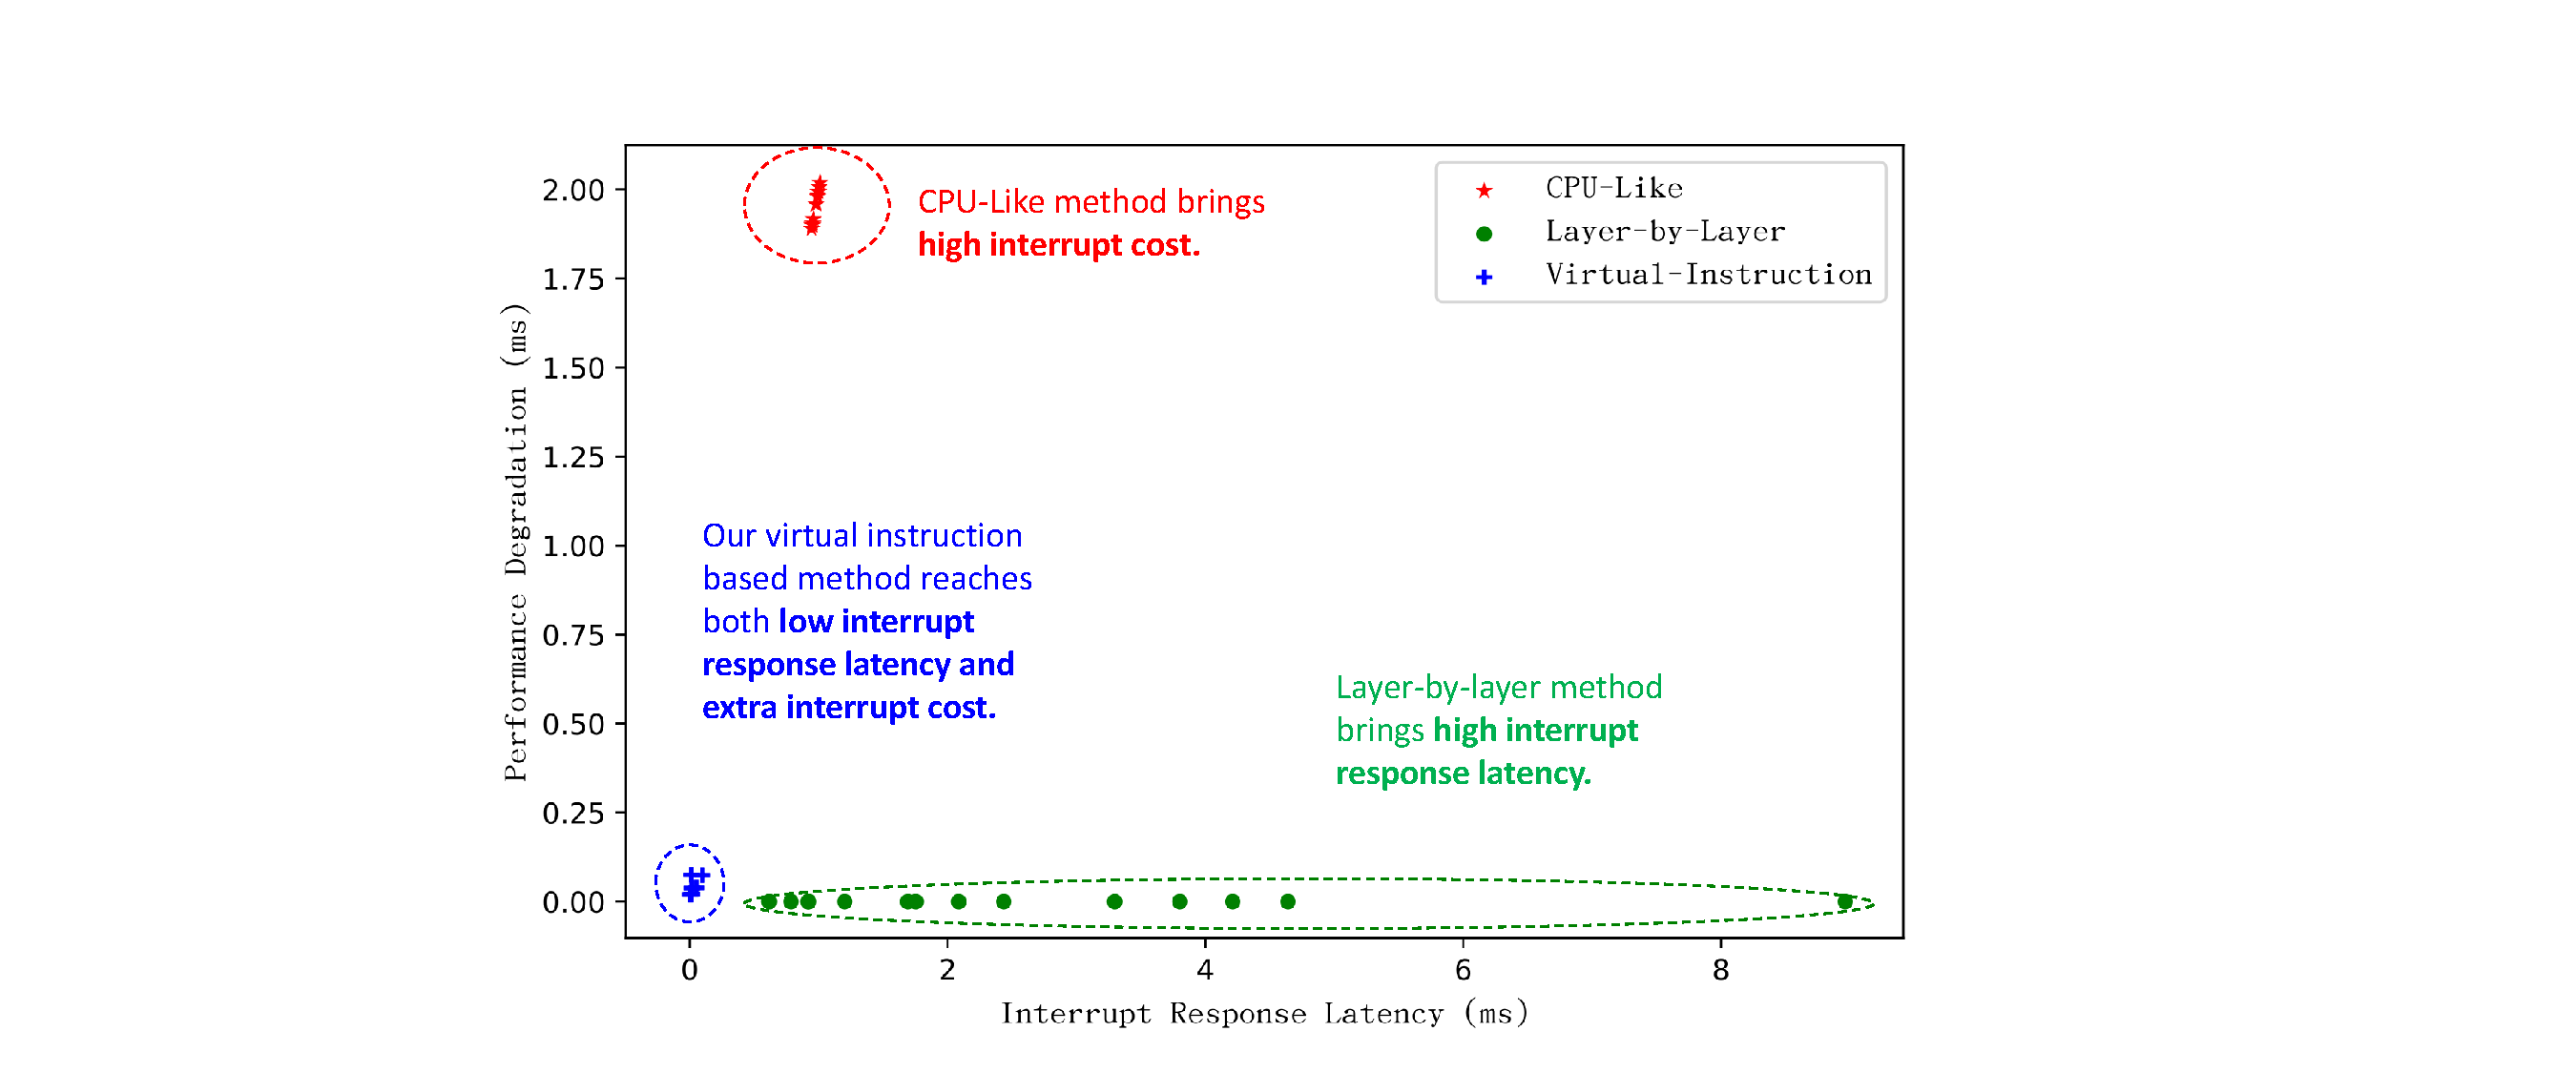
\includegraphics[width=0.9\linewidth]{fig/scatter1024.pdf}
  \caption{The interrupt response latency \& extra time cost for different implementation of interrupt. }
  \label{fig:scatter1024}
\end{figure}

We evaluate the latency to response the interrupt and the performance degradation of different interrupt method. In MR-Exploration, only the low-priority PR task is interruptible, and the interrupt position is unpredictable. Thus, we randomly selected some interrupt locations inside the PR network.

The latency to response the interrupt in CPU-like interrupt includes the time to finish current executing instruction and the data backup time for the on-chip data/weights caches (totally 2.2MB). The latency in layer-by-layer interrupt is the time to finish current layer. The latency of our virtual-instruction-based method is the time to finish current executing instruction and the backup time for the calculated output results. 

The cost of CPU-like interrupt is the data transfer time of all the on-chip caches (totally 2.2MB) to/from DDR. The cost of virtual-instruction-based method is the recovery of the input/weights from DDR to on-chip caches. There is no extra cost fot the layer-by-layer interrupt.

For a precise evaluation the CNN run time, we record the clock cycles of the beginning and end of each instruction. The time of the interrupt response latency and the total cost in the following evaluation is calculated from the clock cycles and the clock frequence.

The CNN backbone of the interruptible PR is ResNet101 \cite{he2016deep}, wich contains 101 convolution layers. The input shapee of the PR CNN is $480 \times 640 \times 3$. The parallelism of the Angel-Eye is $Para_{height}=8$, $Para_{in}=16$, $Para_{out}=16$, i.e. each CALC instruction processes 8 lines from 16 input channe to 16 output channels. 

We randomly sample 12 positions of the ResNet101 CNN backbone. The interrupt response latency and the extra time cost for different implementation of interrupt at the positions are listed in \Cref{fig:scatter1024}.



% The performance and the latency of the interruptible DPU and the not-interruptible DPU are listed in \Cref{tab:anywhere}. 

% We record some of the interrupt locations when running MR-Exploration on the interruptible DPU. 
% \Cref{tab:anywhere} lists the  performance degradation at some typical positions, as well as the worst interrupt response latency of each position. The worst latency in virtual-instruction-based method means the interrupt request occurs at the beginning of a CalcBlob. The worst latency in the layer-by-layer method means interrupt request occurs at the beginning of the Layer.
% The 'Serial' row is the baseline for executing the two tasks in serial without interrupt. 
% In serial execution, backup/recovery of data is not required. The 'CPU-like' row is the estimated result of backup/recovery all the on-chip caches for immediately interruption. The 'Pose 1,2,3' rows are the results of the DPU interrupted at different  PR positions. 'Pose 1' represents the first layers of PR network, the numbers of input channel and output channel are both $64$. The input and output shapes are both $240 \times 320$. 'Pose 2' represents the layers with moderate number of channels ($ 512 $) and data shapes ($ 60 \times 80 $). 'Pose 3' represents the last layers with many channels ($ 2048 $) and small featuremaps ($ 15 \times 20$).

The CPU-like interrupt consumes the most perform degradation. Though the layer-by-layer consumes no extra time, the latency is much higher than our virtual-instruction-based interrupt. In the worst case, the interrupt request occurs at the middle of the most computation consuming layers, whose input shape is $30 \times 40 \times 512$. The kernel shape is $3 \times 3$ and the output shape is also $30 \times 40 \times 512$. The execution time of this layer more than 10ms in the accelerator.
The layer-by-layer interrupt need to wait for the finish of this layer. The performance at same interrupt position in our proposed virtual interrupt is not significantly different from that of other positions. Our method is significantly better than others at worst case. 


\subsubsection{ Additional data transfer for the virtual instructions. }
% The worst latency of the layer-by-layer interrupt reaches 10 ms, because the interrupt occurs at the beginning of the second layer, which is the most time-consuming layer (10ms). The layer-by-layer interrupt need to wait for the finish of this layer. The performance at same interrupt position in our proposed virtual interrupt is not significantly different from that of other positions. Our method is significantly better than others at worst case. 

The extra virtual instruction number is listed in \Cref{tab:instrnum}. Compared to the normal instruction transfer, the volunm of with virtual instructions is less than 10\%. The performance degradation brought by the extra virtual instructions is negligible.



% DPU first calculates all channels of the output row before calculating the next rows. As the number of channels increases, the number of weights requiring recovery increases squarely. However, the size of the input data to be restored and the output results to be backed up remains basically the same.


% % Table generated by Excel2LaTeX from sheet 'Sheet2'
% \begin{table}[t]
%   \small
%   \centering
%   \caption{Worst latency different interrupt positions.}
%     % Table generated by Excel2LaTeX from sheet 'Sheet2'
% \begin{tabular}{|c|c|c|c|c|c|}
%   \hline
%         & Backup  & Recovery & CPU-like & layer-by-layer & Virtual Instr. \bigstrut[t]\\
%         & (KB)  & (KB)  &  Latency (ms) & Latency (ms)   & Latency (ms) \bigstrut[b]\\
%   \hline
%   Pose 1 &       &       &       &      &  \bigstrut\\
%   \hline
%   Pose 2 &       &       &       &      &  \bigstrut\\
%   \hline
%   Pose 3 &       &       &       &      &  \bigstrut\\
%   \hline
%   CPU-Like & 4000  & 4000  &     &       & <1 \bigstrut\\
%   \hline
%   Serial & -     & -     &     &   & - \bigstrut\\
%   \hline
%   \end{tabular}%
  
  
%   \label{tab:anywhere}%
% \end{table}%


% Table generated by Excel2LaTeX from sheet 'Sheet2'
\begin{table}[t]
  \small
  \centering
  \caption{The instruction number of the interruptible PR network. }
    % Table generated by Excel2LaTeX from sheet 'Sheet2'
\begin{tabular}{|c|c|c|c|c|c|}
  \hline
         & Instr.  & Virtual Instr. & Execute \bigstrut[t]\\
        & Number   & Volunm (MB) & Time (ms) \bigstrut[b]\\
  \hline
  Origin   &      364032      & 4.36 & 186.0 \bigstrut\\
  \hline
  Virtual Instr.   &     400243    & 4.79 & 187.2 \bigstrut\\
  \hline
  \end{tabular}%
  \label{tab:instrnum}%
\end{table}%

We are here to reminder the readers that the processing of the low-priority PR task can be interrupted twice or more. And in that case, the PR task is interrupted by several FE tasks.


% % Table generated by Excel2LaTeX from sheet 'Sheet1'
% \begin{table}[t]
%     \centering
%     \caption{Interrupt after complete results vs Interrupt anywhere}
% % Table generated by Excel2LaTeX from sheet 'Sheet2'
% \begin{tabular}{|c|c|c|c|c|c|}
%   \hline
%   \multicolumn{1}{|c}{} &       & \multicolumn{1}{c|}{Backup } & \multicolumn{1}{c|}{Recovery} & Exe time & Performance \bigstrut[t]\\
%   \multicolumn{1}{|c}{} &       & \multicolumn{1}{c|}{data (KB)} & \multicolumn{1}{c|}{ data (KB)} & (ms)  & Reduce \bigstrut[b]\\
%   \hline
%   \multicolumn{1}{|p{3.315em}|}{Inter } & \multicolumn{1}{p{3.69em}|}{AfterSave} &       &       &       &  \bigstrut\\
%   \cline{2-6}\multicolumn{1}{|p{3.315em}|}{position 1} & Anyware &       &       &       &  \bigstrut\\
%   \hline
%   \multicolumn{1}{|p{3.315em}|}{Inter } & \multicolumn{1}{p{3.69em}|}{AfterSave} &       &       &       &  \bigstrut\\
%   \cline{2-6}\multicolumn{1}{|p{3.315em}|}{ position 2} & Anyware &       &       &       &  \bigstrut\\
%   \hline
%   \multicolumn{1}{|p{3.315em}|}{Inter } & \multicolumn{1}{p{3.69em}|}{AfterSave} &       &       &       &  \bigstrut\\
%   \cline{2-6}\multicolumn{1}{|p{3.315em}|}{position 3} & Anyware &       &       &       &  \bigstrut\\
%   \hline
%   \multicolumn{2}{|p{7.005em}|}{CPU-Like} &       &       &       &  \bigstrut\\
%   \hline
%   \multicolumn{1}{|c}{} &       & \multicolumn{1}{c|}{Instruction} & \multicolumn{1}{c|}{Latency} & Exe time & Performance \bigstrut[t]\\
%   \multicolumn{1}{|c}{} &       & \multicolumn{1}{c|}{ (KB)} & \multicolumn{1}{c|}{(ms)} & (ms)  & Reduce \bigstrut[b]\\
%   \hline
%   \multicolumn{1}{|c|}{No} & \multicolumn{1}{p{3.69em}|}{Origin} &       &       &       & 0 \bigstrut\\
%   \cline{2-6}\multicolumn{1}{|c|}{ Interrupt} & \multicolumn{1}{p{3.69em}|}{After results} &       &       &       &  \bigstrut\\
%   \cline{2-6}      & Anyware &       &       &       &  \bigstrut\\
%   \hline
%   \end{tabular}%
  
%     \label{tab:anywhere}%
%   \end{table}%



\subsection{ Place Recognition With the CNN accelerator }

In this section, we design experiments to evaluate the accuracy and efficiency of the PR network on the CNN accelerator. 

\begin{figure}[t]
    \centering
    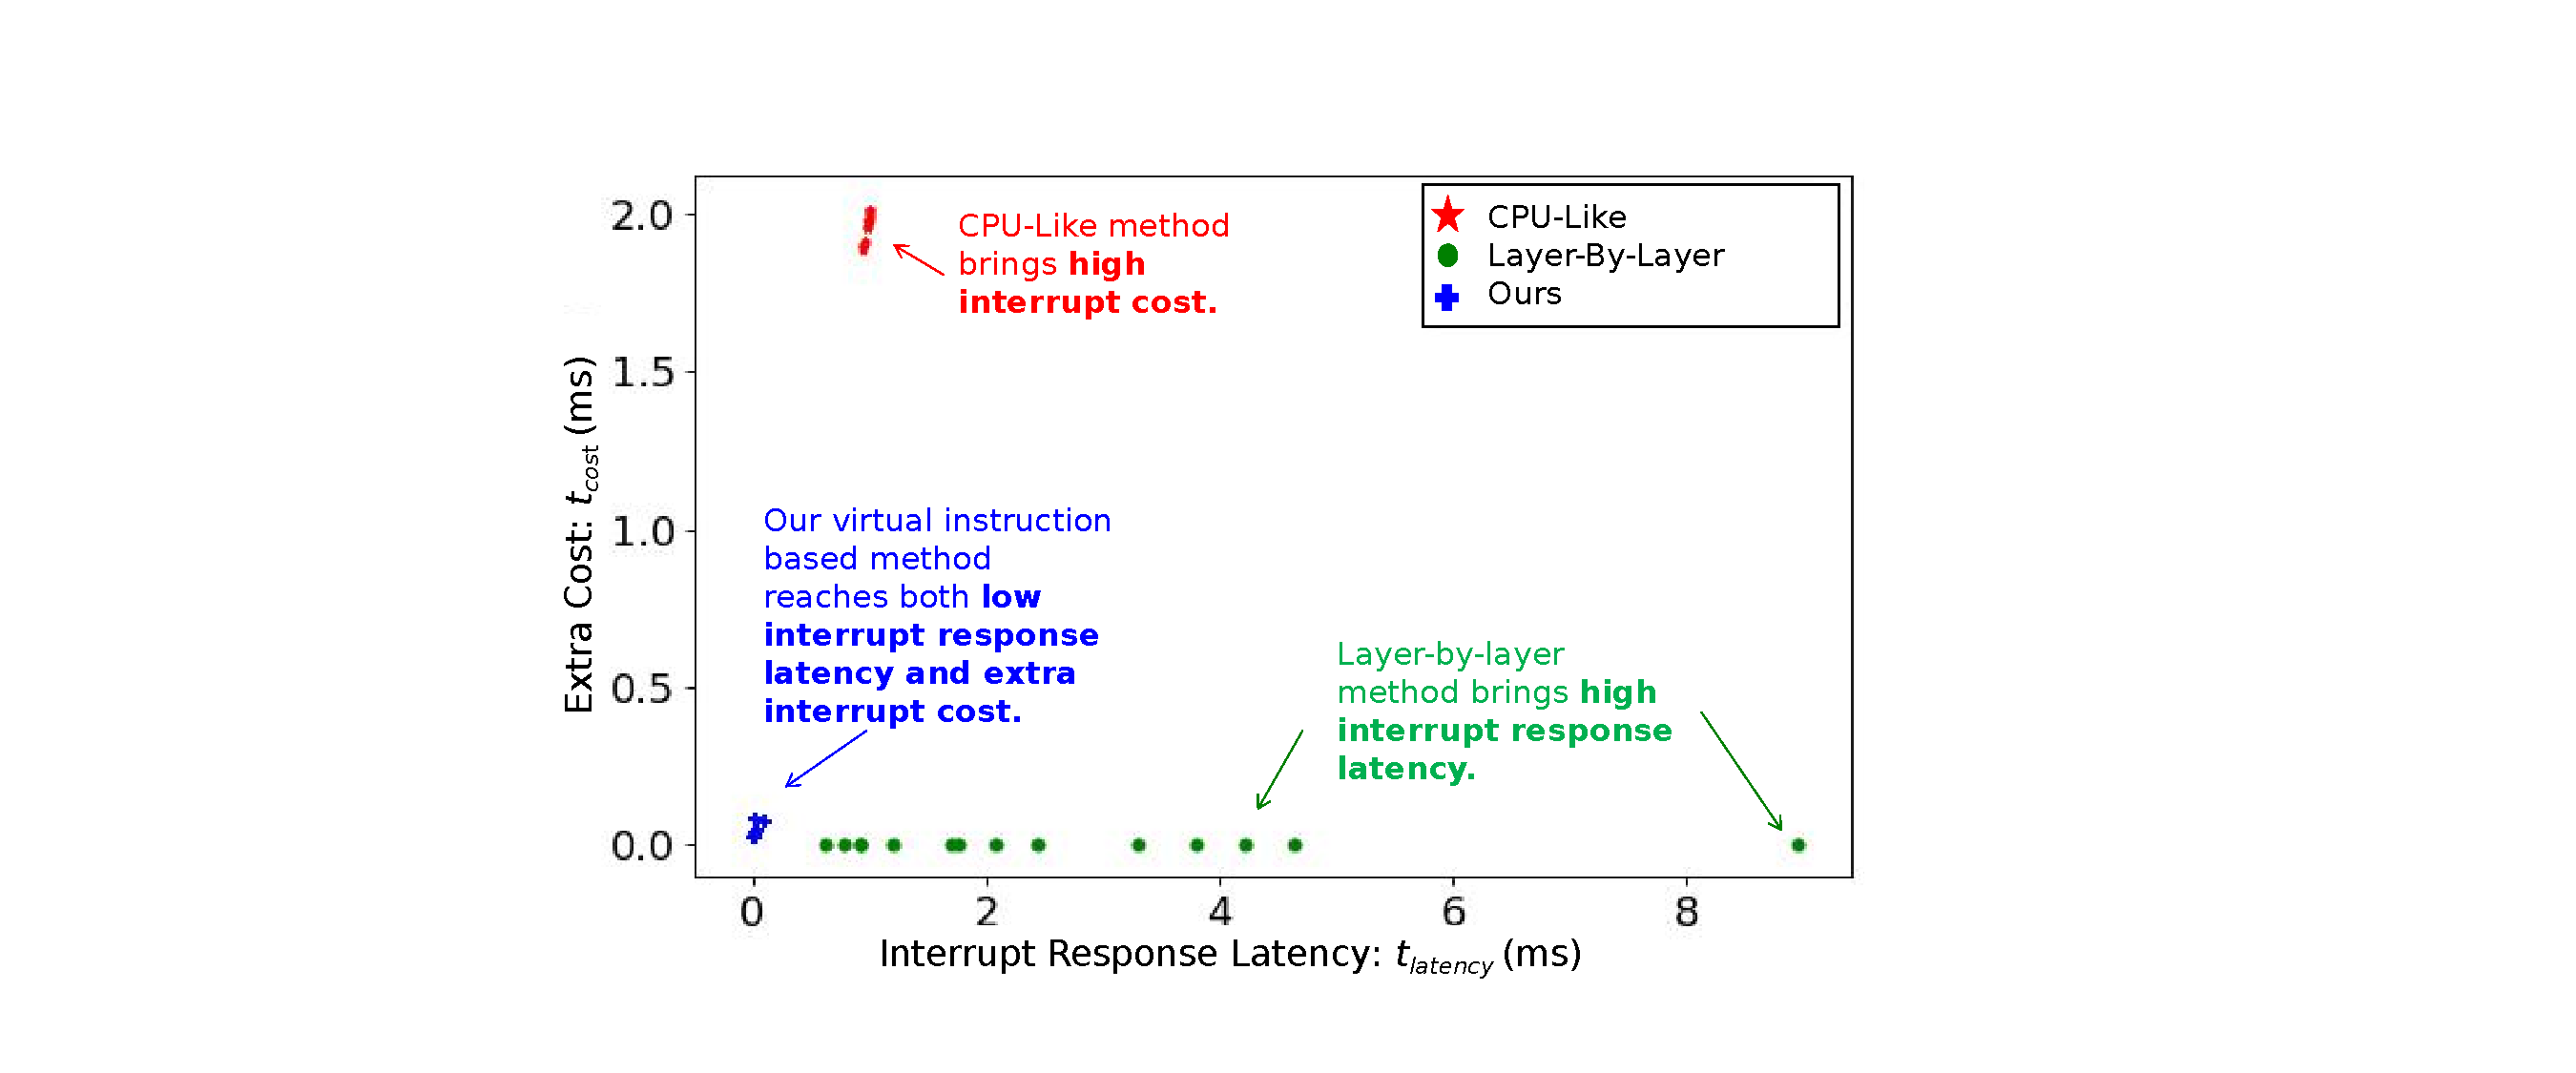
\includegraphics[width=0.8\linewidth]{fig/PRresult.pdf}
    \caption{Precision-Recall curve on Citycenter dataset}
    \label{fig:PRcurve}
\end{figure}

We want to prove two things in our experiment. 1) The GeM network used in our work outperforms other networks such as NetVLAD. 2) The quantization of GeM CNN backbone don't bring about much drop in accuracy. We test 3 networks, a) float-point GeM, b) float-point NetVLAD, c) fixed-point GeM on Citycenter dataset and draw the Precision-Recall curve. The result is shown in figure \ref{fig:PRcurve}. It's clear that float-point GeM netowrk run better than NetVLAD in all situations. After quantization, the accuracy goes down a bit, especially when precision is high. But the quantized network still outperforms NetVLAD in most cases.

% \begin{figure}[t]
%   \centering
%   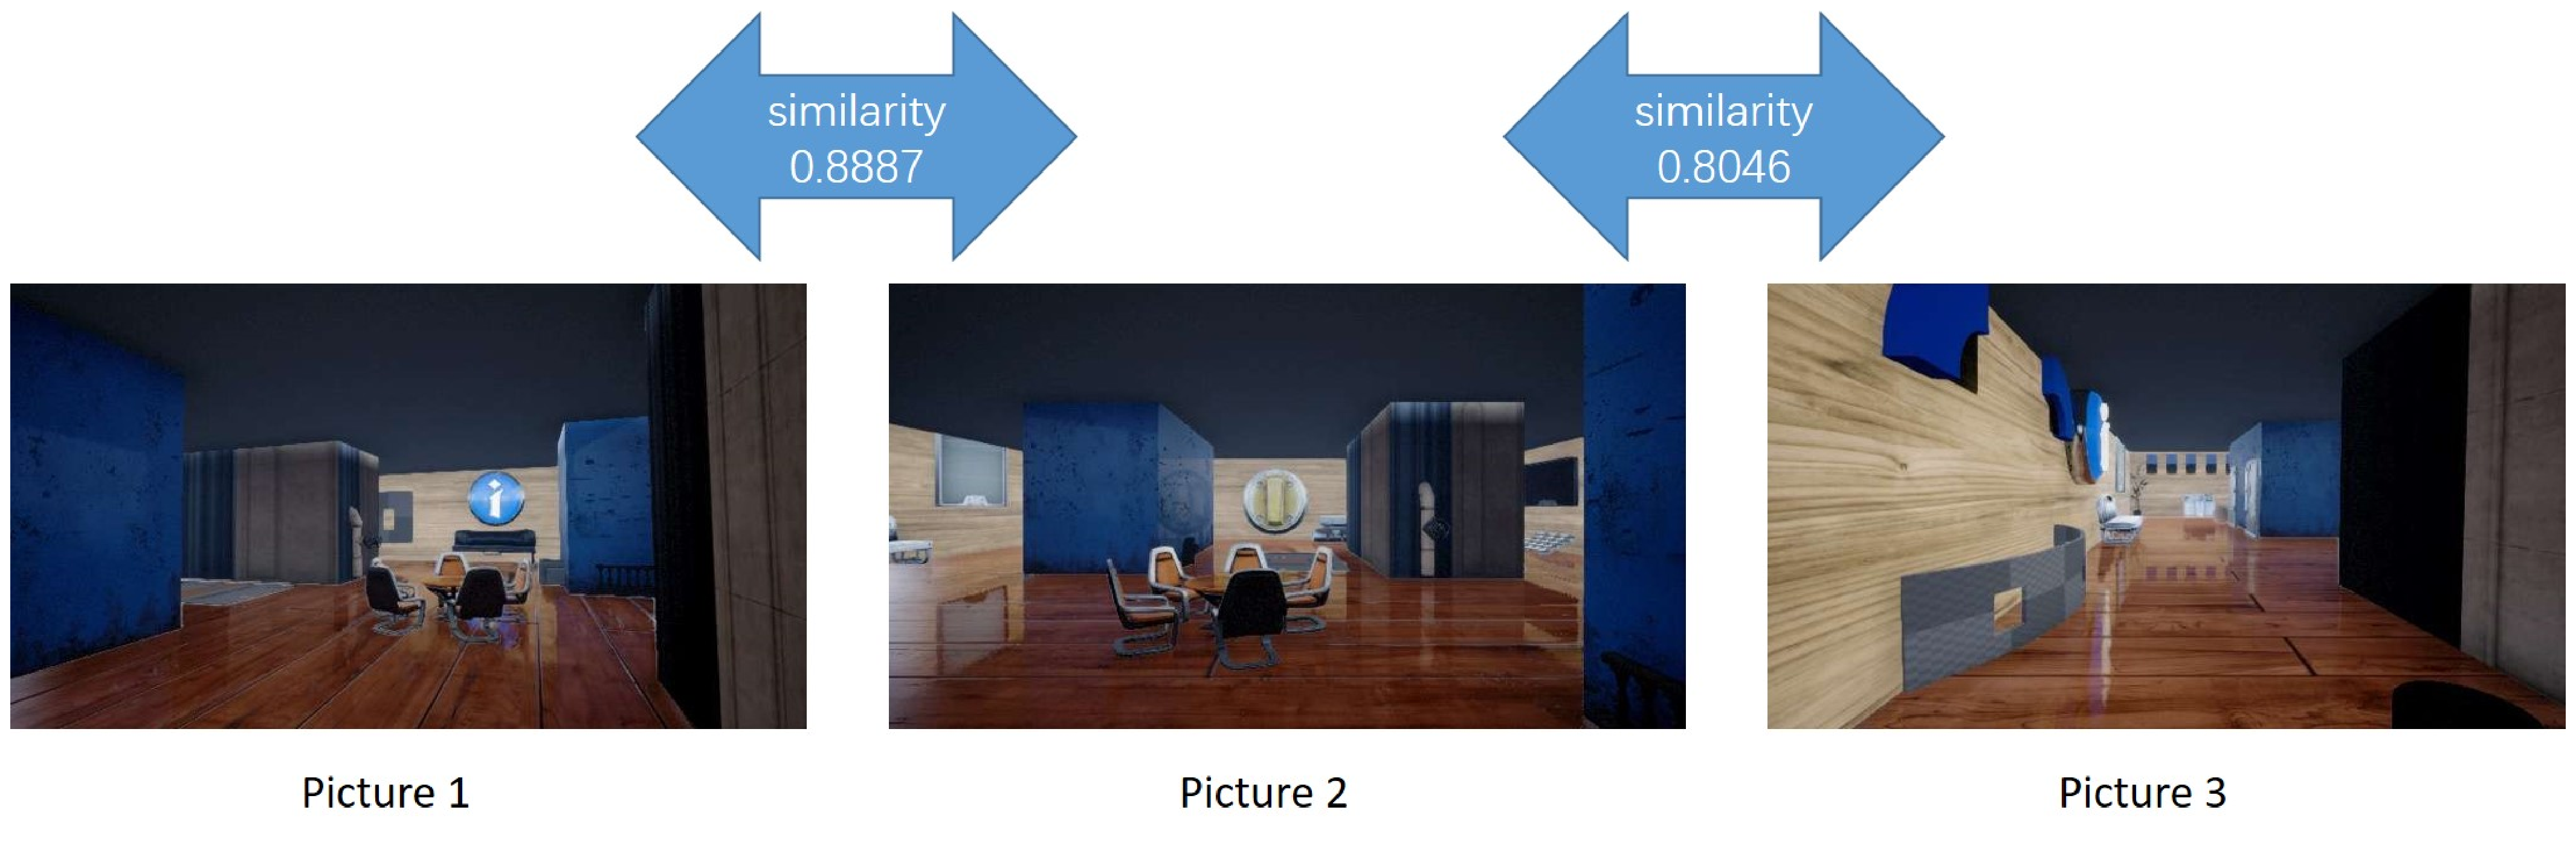
\includegraphics[width=0.8\linewidth]{fig/example.eps}
%   \caption{Example of GeM performance.}
%   \label{fig:gem_exp}
% \end{figure}

% Figure \ref{fig:gem_exp} shows an example in our similation environment. Picture 1 and Picture 2 is photoed in the same place and Picture 3 is photoed in another place. The computed similarity of Picture 1 and 2 is 0.8887, apparently larger than the similarity of Picture 2 and 3 (0.8046).

% \subsubsection{efficiency}

% \begin{table}
%     \label{tab:gem_eff}
%     \centering 
%     \caption{runtime comparison of each operation in PR}
%     \begin{tabular}{|c|c|c|}
% 				\hline
%               & CPU & CPU+FPGA \\
%         \hline
%            &   48 ms &   42 ms \\
% 			  \hline
%     \end{tabular}
%   \end{table}

% As illustrated in section \ref{sec:hardsoftcodesign}, we do optimization on GeM backend processing, i.e., the GeM pooling layer. We compare running time before and after optimization, and the result is shown in table \ref{tab:gem_eff}. After optimization, the total time reduces by 12.5\%.


\subsection{ Feature-point Extraction With the CNN accelerator }

To evaluate the performance of the SuperPoint network in visual odometer, we experimented on the $TUM$ dataset. We evaluate SuperPoint against two well-known FE systems: SIFT\cite{Lowe-478} and ORB\cite{RubleeRabaud-479}. We apply the three systems to the visual odometer. We also evaluate the performance after optimization. We compute a maximum of 200 points for all systems at a $480\times640$ resolution and set $NMS=4$. We perform nearest neighbor matching from descriptors in adjacent frames with a maximum allowable distance $d_m$. $d_m$ is not same in three system because descriptors are not in the same order of magnitude. We use an OpenCV implementation (solvePnP()) with all the matches to compute the transform matrix \cite{LepetitMoreno-Noguer-EPnP}, and use Bundle Adjustment to optimize results \cite{TriggsMclauchlan-Bundle-Adjustment}. All the computation of this experiment is all done on the CPU except CNN of SuperPoint. 

\begin{table}[t]
  \centering
  \caption{ Accuracy and runtime results on the TUM\cite{sturm12iros} SLAM dataset  }
  \footnotesize
  \begin{threeparttable}
% Table generated by Excel2LaTeX from sheet 'Sheet2'
\begin{tabular}{|c|c|c|c|c|} 
  \hline
        & \multirow{2}[2]{*}{$d_m$$^1$} & RPE$^2$ & ATE$^3$  & Run  \bigstrut[t]\\
        &       &  (m/s) & (m) & time(ms) \bigstrut[b]\\
  \hline
  SIFT  & 200   & 0.0319  & 0.4219 & 2397  \bigstrut\\
  \hline
  ORB   & 30    & 0.0577  & 0.6105 & 229  \bigstrut\\
  \hline
  Origin & \multirow{2}[2]{*}{0.7} & \multirow{2}[2]{*}{0.0280} & \multirow{2}[2]{*}{0.3671} & \multirow{2}[2]{*}{259} \bigstrut[t]\\
   Superpoint &       &       &       &  \bigstrut[b]\\
  \hline
  Our Fixed & \multirow{2}[2]{*}{360} & \multirow{2}[2]{*}{0.0283} & \multirow{2}[2]{*}{0.3976} & \multirow{2}[2]{*}{59} \bigstrut[t]\\
   Superpoint &       &       &       &  \bigstrut[b]\\
  \hline
  \end{tabular}%
  

\begin{tablenotes}
  \item[1] $d_m$ is the maximum allowable distance between matched descriptors.  
  \item[2] RPE is the mean Relative Pose Error to indicate the translational drift per second, the less, the better.
  \item[3] ATE is the root mean square Absolute Trajectory Error to indicate the translational drift of the entire trajectory, the less, the better.
\end{tablenotes}
    \end{threeparttable}
  \label{tab:VO}%
\end{table}%

Results are shown in \Cref{tab:VO}. In terms of accuracy, SuperPoint outperforms ORB and performs comparably to SIFT. Optimization does not introduce a large loss of accuracy. In terms of calculation speed, SuperPoint takes less time than Sift, and is equivalent to Orb. After optimization, the running speed is increased by $4\times$, making real-time processing possible.

\begin{table}[t]
  \centering
  \caption{runtime Comparison of each operation}
% Table generated by Excel2LaTeX from sheet 'Sheet2'
\begin{tabular}{|c|c|c|c|c|}
  \hline
             &    softmax &        NMS &       rank &  normalize \bigstrut\\
  \hline
         CPU &       31ms &       27ms &       0.97ms &       42ms \bigstrut\\
  \hline
    CPU+FPGA &     1.97ms &      0.7ms &     0.12ms &     1.44ms \bigstrut\\
  \hline
  \end{tabular}  
  
  \label{tab:optimization}%
\end{table}%

We compare the running time of each operation in SuperPoint before and after the optimization. Results are shown in \Cref{tab:optimization}. The running time of each operation is reduced by more than $20\times$. There is a certain gap between the experimental results of the acceleration effect and the theoretical derivation in \Cref{subsec:FEopt}. The possible reason is that the CPU needs time to schedule the FPGA accelerator.

\subsection{ ROS based MR-Exploration }

The results of the Multi-Robot Exploration based on our INCAME is shown in \Cref{fig:env}. The space in the AirSim for the robots to explore is shown in \Cref{fig:env}(a). It is a simple rectangle area with four different pillars, and some chairs at the center (in the white box).  \Cref{fig:env}(b) shows how PR works for map maerging. The FE and VO on each agent produce the local map and trajectory on each ZCU102 board. When the PR threads on different agents find out a similar scene. The relative pose of the two agents at the similar scene are calculated. The map and the trajectory is merged with the calculated relative pose, as shown in \Cref{fig:env}(c).

In this example, the FE and PR are both executed on the same Angel-Eye accelerator. The frequence of the input camera is 20fps, and each input frame is fed to the FE, and FE module would take up accelerator. While the CPU process VO with the feature-points from FE, the accelerator can switch to process the low-priority PR task. Because the executing time of VO varies, the time to finish a PR task is different. In this example, the time from the begin a PR to its end is 320~500 ms. Thus, the PR samples one frame from every 7$\sim$10 frames.